% Chapter 1
\chapter{Getting started}

% Overview
\section{Overview}

To begin with, you should know what \IzPack is organized if you want to use
it. Let's go into the directory where you have installed \IzPack on your
machine. There are 3 text files and a set of directories. The most
important for the moment are \texttt{bin/ doc/ sample/}. If you are reading this,
you already know that \texttt{doc} contains this documentation :-)\\

So let's go into \texttt{bin/}. The \texttt{icons/} directory contains some
directories for your system, in case you would like an icon to launch a
component of \IzPack. But the most important things you can see in \texttt{bin}
are the texttt{compile} scripts (in both Unix* and Windows formats).
\texttt{compile} is used to compile a ready-to-go XML installation file from
a command-line context or from an external tool.\\

\noindent
\textit{Note : these scripts can be launched from anywhere on your system as the
installer has customized these scripts so that they can inform \IzPack of where
it is located.}\\

% First Compilation
\section{First Compilation}

Now you probably can't wait to build your first installer. So go on open a
command-line shell and navigate to \texttt{sample/}. The following should work
on both Unix* and Windows systems. For the latter, just change the path
separator (slash '/') to a backslash. So type (\$ is your shell prompt !) :
\begin{verbatim}
$ ../bin/compile install.xml -b . -o install.jar -k standard
 (installer generation text output here)
$ java -jar install.jar
\end{verbatim}

There you are! The first command has produced the installer and the
second one did launch it.

% The IzPack Architecture
\section{The \IzPack Architecture}

Now that you have packaged your first installer, it's time for you to understand
how the whole thing works.\\

\subsection{The Compilation System}

The compilation system (see figure \ref{comparch}) is quite modular. 
Indeed, you can use the compiler in 3 ways :
\begin{itemize}
  \item from a command-line
  \item from Jakarta Ant
\end{itemize}\

\begin{figure}[h]
\caption{\label{comparch}
         \textit{The compiler architecture.}}
\begin{center}
\fbox{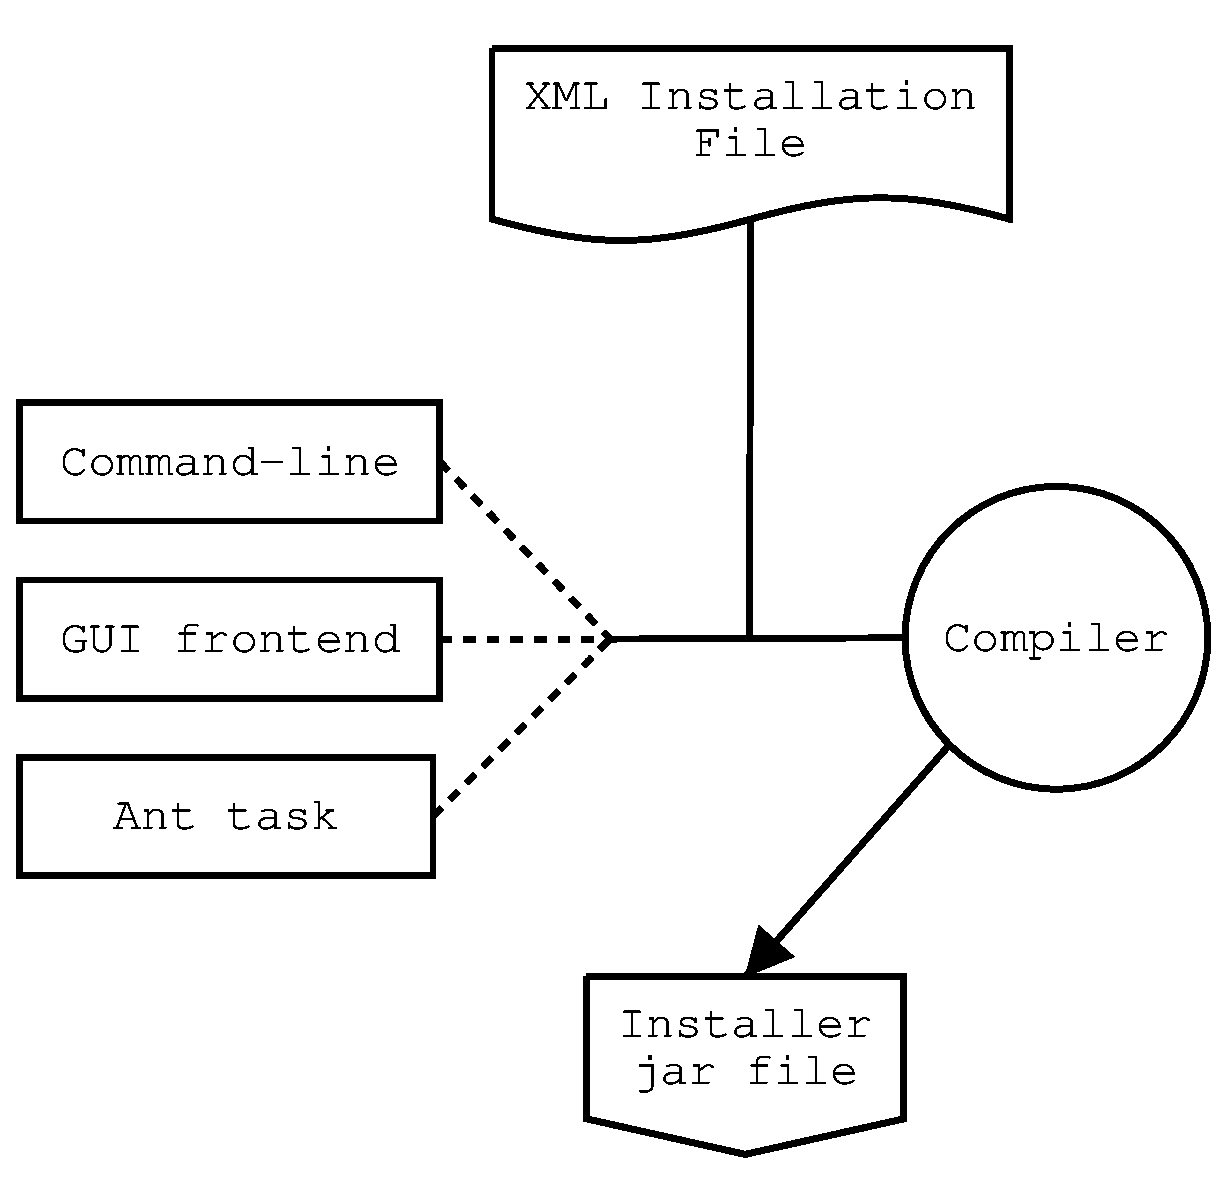
\includegraphics[scale=0.4]{img/ch1-comparch}}
\end{center}
\end{figure}

The compiler takes as its input an XML installation file that describes
(at a relatively high-level) the installation. This file contains
detailed information such as the application name, the authors, the
files to install, the panels to use, which resources to load and much
more (see figure \ref{archinstaller}).\\

The compiler can generate different kinds of installers, but this information is
not located inside the XML file as it is not were it should be. On the contrary,
this is a compiler parameter.\\

The compilation options for a command-line installer are the following:
\begin{itemize}
\item \texttt{-?}: gives a list of the available options.
\item \texttt{-b}: specifies the base path, \textsl{ie} the one that will be
used to resolve the relative paths. If your XML file contains absolute paths,
specify it to an empty string (\texttt{-b ""}).
\item \texttt{-k}: specifies the installer kind, for instance most users will
want \texttt{standard} here.
\item \texttt{-o}: specifies the resulting installer Jar file name.
\end{itemize}\

\subsection{How an Installer Works}

An installer presents its panels to the end-user. For instance, there is
one to select the packages, one to prompt for the license agreement, one
to select the installation path and so on. You have a choice from a
variety of panels to place in the installer. For example, you can choose
between a plain text and a HTML text panel for the license agreement.
Also, if you don't want of the \textit{HelloPanel}, you just don't
include it.\\ 

\begin{figure}[h]
\caption{\label{archinstaller}
         \textit{The installer architecture.}}
\begin{center}
\fbox{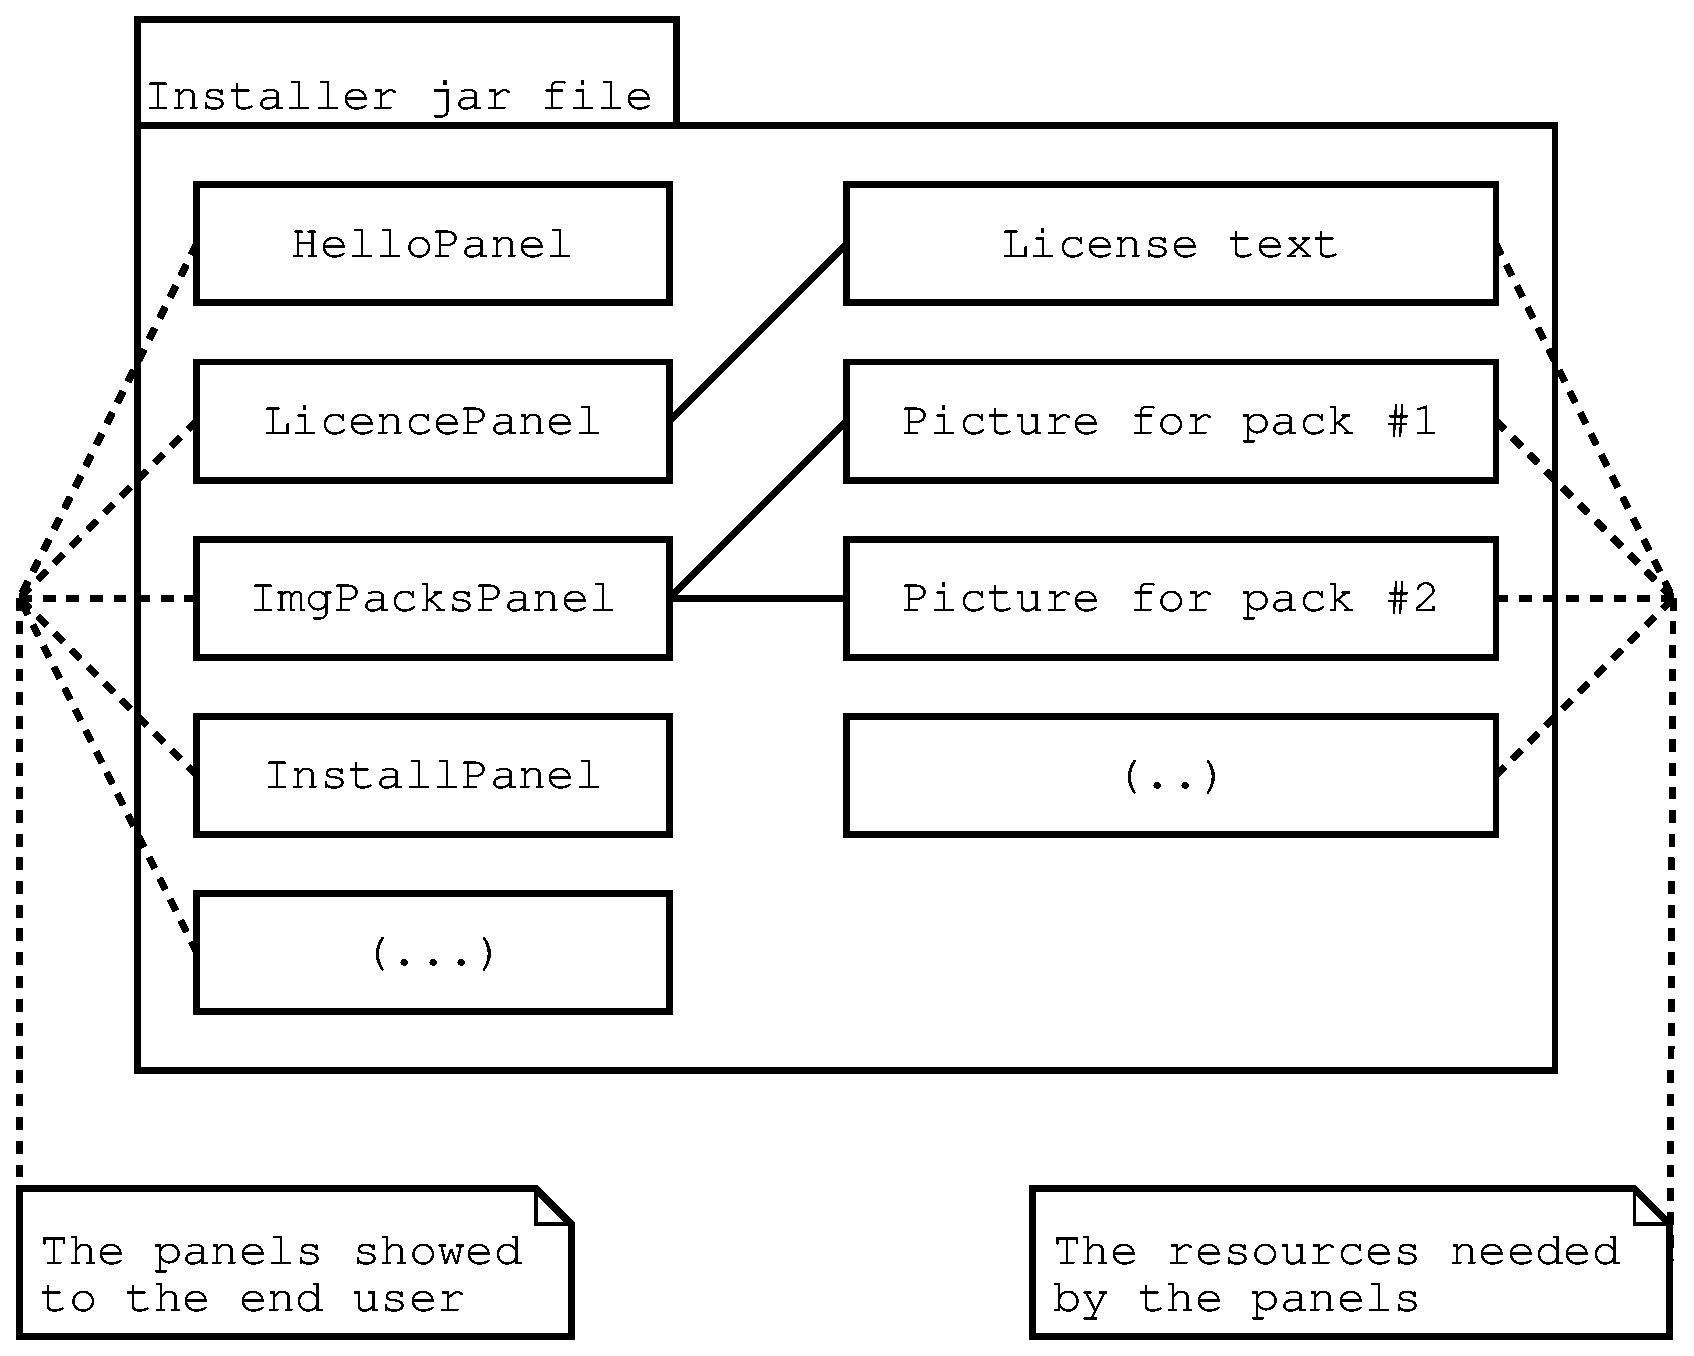
\includegraphics[scale=0.4]{img/ch1-compinside}}
\end{center}
\end{figure}

It is very important to understand that some of the panels may need extra data. For
instance, the license agreement panel needs the license text. A simple approach
to specify such data would have been to add as many XML tags as needed for
each panel. However, this makes the XML file too specific and not easy to
maintain. The approach that has been chosen is to put the data in files and we
call these files \textit{resource files}. They are specified with a unique XML
tag. This is a much cleaner approach.\\

You might wonder how your files are packaged. They can be grouped in
\textit{packs}. For instance, you can have one pack for the core files, one for
the documentation, one for the source code and so on. In this way, your end-users
will have the choice to install a pack or not (provided that the pack they don't
want to install is not mandatory). Inside the jar file (which is a zip file), a
sub directory contains the pack files. Each pack file contains the files that are
part of it. Could we do it simpler ? :-)\\

\subsection{The Different Kinds of Installers}

There are for the moment 4 kinds of installers available :
\begin{itemize}

  \item \texttt{standard} : a single-file ready-to-run installer
  \item \texttt{standard-kunststoff} : same as above but using the Kunststoff
  Look and Feel
  \item \texttt{web} : a web based installer (the packs files are located on a
  HTTP server and the user installer will fetch it for him)
  \item \texttt{web-kunststoff} : same as above but using the Kunststoff
  Look and Feel.

\end{itemize}\
